\chapter{Feedback linearization}
Given a nonlinear system of the following form
\[
\begin{cases}
	&\dot{x}=a(x)+b(x)u\\
	&y=c(x)
\end{cases}
\]
design a static state feedback control law $u=k(x,v)$ such that the associated feedback system is linear. Let's purse this goal looking at an example.
\section{Introductory example}
\begin{figure}[H]
	\centering
	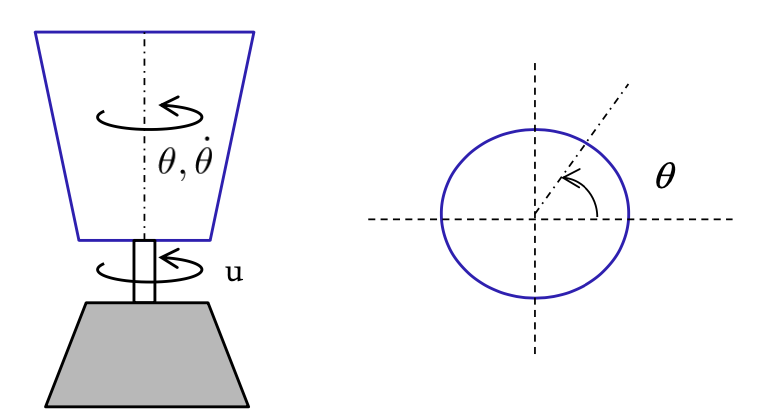
\includegraphics[scale=0.4]{immagini/frullatore}
	\caption{Centrifuge}
	\label{fig:frullatore}
\end{figure}
	We want to build the speed regulator of a centrifuge modeled as follows:\[J\ddot{\Theta}=-k\dot{\theta}^2sgn(\dot{\theta})+u\]
	Where $J\ddot{\theta}$ is the moment of inertia which is equal to the sum between the friction torque proportional to the square of the angular velocity and the torque control input.\\
	Setting $y=x=\dot{\theta}$ (speed control), we get 
	\[\begin{cases}
		&\dot{x}=-\frac{k}{J}x^2sgn(x)+\frac{1}{J}u\\
		&y=x
	\end{cases}
\]
If we set $v\colon =-\frac{k}{J}x^2sgn(x)+\frac{1}{J}u \Leftrightarrow u=-kx^2sgn(x)+Jv$ then we get the feedback linear system $S^*$: \[\begin{cases}
	&	\dot{x}=v\\&y=x
\end{cases}\]\begin{figure}[H]
\centering
\includegraphics[scale=0.4]{immagini/Sstar}
\caption{Feedback linear system}
\label{fig:s}
\end{figure}
So now we have $G(s)=\frac{1}{s}$ and it is possible to design a rotational speed controller by the pole assignment method for linear systems.\begin{figure}[H]
	\centering
	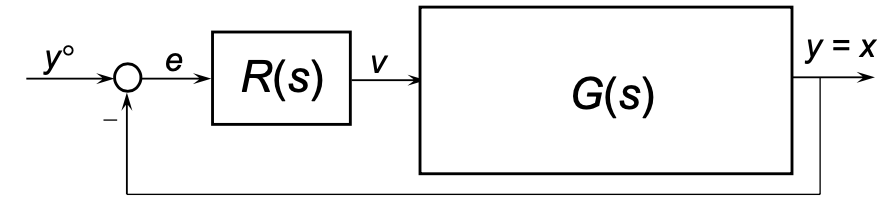
\includegraphics[scale=0.4]{immagini/examplefeed}
	\label{fig:examplefeed}
\end{figure}
We can adopt a static proportional controller: $v=k_pe$ with $e=y°-y$ so the resulting transfer function from y° to y is given by $F(s)=\frac{k_p\frac{1}{s}}{1+k_p\frac{1}{s}}=\frac{1}{1+\frac{s}{k_p}}$.
\begin{figure}[H]
	\centering
	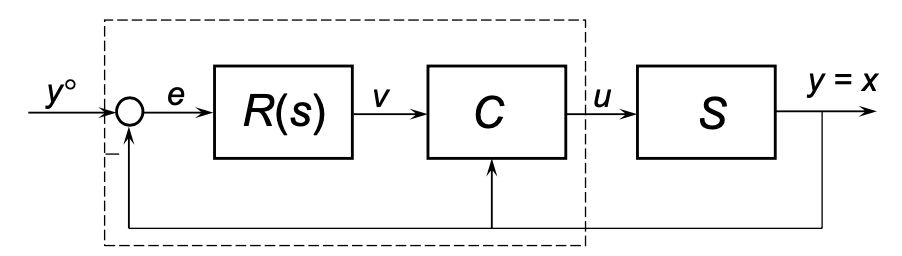
\includegraphics[scale=0.4]{immagini/feedbackcontrollerex}
	\caption{Controller}
	\label{fig:feedbackcontrollerex}
\end{figure}
In the end the designed nonlinear controller is: \[
u=-kx^2sgn(x)+Jk_p(y°-x)
\]
Now the question we have to pose ourselves are:
\begin{itemize}
	\item Under what conditions there exists a static feedback control law that makes the feedback system linear?
	\item How can one design state feedback linearization?
\end{itemize}
\section{Fully linearizable system}
Let us consider a nonlinear system in the so-called normal form:
\[
\begin{cases}
	\dot{x}_1=x_2\\
	\dot{x}_2=x_3\\
	\dot{x}_3=x_4\\
	\dot{x}_4=\phi(x_1,x_2,x_3,x_4)+bu\\
	y=x_1
\end{cases}\qquad x=\begin{bmatrix}
x_1\\x_2\\\vdots\\x_n
\end{bmatrix}
\] where $\phi(\cdot,\cdot,\cdot,\cdot)$ is a known nonlinear function and $b\neq0$ we just need to set $u=\frac{1}{b}(-\phi(x)+v)$ in order to obtain a linear feedback system.
\[
\begin{cases}
	\dot{x}_1=x_2\\
	\dot{x}_2=x_3\\
	\dot{x}_3=x_4\\
	\dot{x}_4=v\\
	y=x_1
	\end{cases}\] So we can state that 
\begin{tcolorbox}[colframe=red!50!white, arc=0mm, colback=white]
	If we can rewrite the system in the above noraml form via a suitable change of state variables, then the system is \textcolor{red}{fully linearizable} via a static state feedback $\rightarrow$ \textcolor{red}{input/state linearization}
\end{tcolorbox}
\section{Partially linearizable system}
Let us consider a nonlinear system in the normal form
\[
\begin{cases}
	\dot{\xi}_1=\xi_2\\
	\dot{\xi}_2=\xi_3\\
	\vdots\\
	\dot{\xi}_r=a_{\xi}(\xi,\eta)+b(\xi,\eta)u\\
	\dot{\eta}=a_{\nu}(\xi,\eta)\\
	y=\xi_1
\end{cases}
\qquad \qquad
x=\begin{bmatrix}
	\xi\\\eta
\end{bmatrix}
\] where $b(\xi,\eta)\neq0$. If we set $u=\frac{1}{b(\xi,\eta)}(-a_{\xi}(\xi,\eta)+v)$ the resulting feedback system is still nonlinear, and appears as follow:
\[
\begin{cases}
	\dot{\xi}_1=\xi_2\\
	\dot{\xi}_2=\xi_3\\
	\vdots\\
	\dot{\xi}_r=v\\
	\boxed{\dot{\eta}=a_{\nu}(\xi,\eta)}\qquad \leftarrow\text{nonlinear dynamics}\\
	y=\xi_1
\end{cases}
\] with a linear I/O map given by the differential equation $\frac{d^ry}{dt^r}=v$ or, equivalently, by the transfer function $G(s)=\frac{1}{s^r}$.\\The system is \textcolor{red}{partially linearizable} via the state feedback control law  $u=\frac{1}{b(\xi,\eta)}(-a_{\xi}(\xi,\eta)+v)$ and the external dynamic is linearized by state feedback $\rightarrow$ \textcolor{red}{input/output linearization}.\\If we set all the state variable equal to zero at the origin $v(\cdot)=0, \xi_1(0)=\xi_2(0)=\dots=\xi_r(0)$, then $y(\cdot)=0$. Correspondingly, $\xi_1(\cdot)=\xi_2(\cdot)=\dots=\xi_r(\cdot)$, while $\eta$ evolves according to $\dot{\eta}a_{\eta}(0,\eta),\eta(0)=\eta_0$ (no zero-state observability). This hidden dynamics is called \emph{zero dynamics}.
\begin{tcolorbox}[colframe=red!50!white, arc=0mm, colback=white]
If the system can be rewritten in the normal form by a suitable state coordinate transformation, then, it is \textcolor{red}{input-output linearizable} via static state feedback.
But... one must consider the behaviour of the \textcolor{red}{zero dynamics}!
\end{tcolorbox}Making a point of what we are doing, we are considering a nonlinear system affine in the input of the following form \[\text{S}: \begin{cases}
\dot{x}(t)=a(x(t))+b(x(t))u(t)\\
y(t)=c(x(t))
\end{cases}
\] we want to design a static state feedback control law $u=k(x,v)$ such that the associated feedback system is linear.
\begin{remark}
		This procedure is different from the approximation of a nonlinear system via the tangent model around some trajectory/equilibrium.\\
		The theory developed is for a nonlinear system affine in the input, not a general system like $\begin{cases}
			\dot{x}=f(x,u)\\y=c(x)
		\end{cases}$ but one can add an integrator and enlarge the state to get a nonlinear system which is affine in the input. And in general having an integrator is good for good tracking performance.

\end{remark}
\section{State feedback linearization}
Given a nonlinear affine system, time-invariant, SISO:
\[\text{S}: \begin{cases}
	\dot{x}(t)=a(x(t))+b(x(t))u(t)\\
	y(t)=c(x(t))
\end{cases}
\] we need some \textbf{regularity assumptions} on system S:\\ $a(\cdot),b(\cdot),c(\cdot)$ should be such that exists a unique evolution associated to any piecewise continuous input u, and continuously differentiable for any order (of class $C^\infty$). \\
In order to understand how to say if a system is fully or partially state feedback linearizable we have to introduce the notion of \textcolor{red}{relative degree}.
\paragraph{Relative degree}
\begin{defn}[Relative degree]
	The relative degree \emph{r} of a system S is given by the minimum order of the time derivative of the output \emph{y} that is affected directly by the input \emph{u}.
\end{defn}
We have to compute the derivatives of the output and progressively increase the order of derivation \emph{k} till we get the (smallest) \emph{k} such that \[y^{(k)}\colon=\frac{d^ky}{dt^k}\] depends directly on the input u.\\We need first to introduce some notations and concepts.
\begin{defn}[Regular functions]
	Let A be on open subset of $\Re^n$ and \emph{f} a real function defined on A\[f\colon A\to\Re\]\\ Function \emph{f} is \emph{regular in $x \in A$} if it is continuously differentiable of any order in $x\colon f \in C^\infty$.\\Function f is \emph{regular in A}, if it is regular in every point of A.\\The vector-value function $f=\begin{bmatrix}
			f_1 & f_2 & \dots & f_m
		\end{bmatrix}'\colon A \to \Re^m$ is \emph{regular} if all functions in f are regular , and it is then called \emph{regular vector field defined on A}.
\end{defn}
\begin{defn}[Jacobian]
	The Jacobian of $f=\begin{bmatrix}
		f_1 & f_2 & \dots & f_m
	\end{bmatrix}'$ is the following matrix of functions 
\[
f_x\colon=\frac{\partial f}{\partial x}=
\begin{bmatrix}
	\frac{\partial f_1}{\partial x_1} & \frac{\partial f_1}{\partial x_2} & \dots & \frac{\partial f_1}{\partial x_n}\\
	\frac{\partial f_2}{\partial x_1} & \frac{\partial f_2}{\partial x_2} & \dots & \frac{\partial f_2}{\partial x_n}\\
	\dots & \dots & \dots & \dots \\
	\frac{\partial f_m}{\partial x_1} & \frac{\partial f_m}{\partial x_2} & \dots & \frac{\partial f_m}{\partial x_n}
\end{bmatrix}
\] We shall denote its value at some x° with $\frac{\partial f}{\partial x}(x°) \text{or} [f_x]_{x°}$.
\end{defn}
\begin{defn}[Lie Derivative]
	Let A be an open set in $\Re^n$ and $f\colon A \to \Re^n$ a regular vector field on A. The \emph{Lie derivative along the vector field} is the operator 
	\[
	L_f\colon=\sum_{i=1}^{n}f_i(x)\frac{\partial}{\partial x_i}
	\]
Given a regular vector field $h\colon A\to 	\Re^m$, the Lie derivative of h along the vector field f is given by: \[
\boxed{L_fh=h_xf\colon A\to \Re^m}
\]
\end{defn}
\begin{remark}
	We have already seen it when computing the time derivative of a Lyapunov function V(x) along the trajectories af a system
	\[\dot{x}=f(x)\to\dot{V}(x)=\sum_{i=1}^{n}f_i(x)\frac{\partial V}{\partial x_i}=V_xf=L_fV\]
\end{remark}
If we iterate the Lie derivative along f we get \[L_f^2h\colon=L_f(L_fh)\] In general \[L_f^kh\colon=L_f(L_f^{k-1}h),\quad L_f^0h=h.\]
Given a regular vector field $g\colon A\to \Re^n$ 
\[
L_gL_fh=\frac{\partial (L_fh)}{\partial x}g
\]
\\
We are now ready to compute the relative degree of S in $x°\in \Re^n$, by determining the derivatives of the output y.
\begin{itemize}
	\item First order time derivative of y: \[\dot{y}=c_x\dot{x}=c_x(a+bu)=L_ac+uL_bc\] If $[L_bc]_{x°}\neq 0$, then $[L_bc]_{x°}\neq 0$ in a neighborhood of x° (by the regularity assumption on S) and we can conclude that the relative degree of S in x° is r=1.\\
	\\
	If $[L_bc]_{x°}=0$, then, the relative degree r of S in x° is either not well-defined or is larger then 1.
	\item If $[L_bc]_{x°}=0$ but in a neighborhood of x° there is some x such that $[L_bc]_{x}\neq 0$, then the relative degree of S in x° is not well-defined.
	\begin{figure}[H]
		\centering
		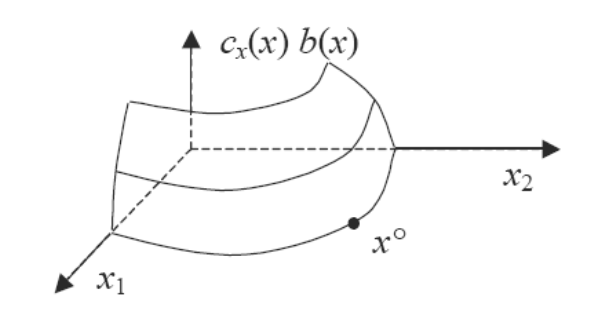
\includegraphics[scale=0.4]{immagini/neighborhood}
		\label{fig:neighborhood}
	\end{figure}
	\item If $[L_bc]_x=0$ in some neighborhood of x°, then we have to take the second order derivative to determine r.
	\item Let $[L_bc]_{x°}=0$ in some neighborhood of x°, that is $\dot{y}=L_ac$.\\Second order time derivative of y: \[\ddot{y}=\frac{\partial L_ac}{\partial x}(a+bu)=L_a^2c+uL_bL_ac\]
	If $[L_bL_ac]_{x°}\neq 0$, then, r = 2.\\
	If $L_bL_ac \equiv 0 $ in some neighborhood of x°, then r>2 (otherwise r is nor well-defined in x°), $\ddot{y}=L_a^2c$, and we need to move on the third order time derivative o$y^{3}$
	\item By iterating this producer, if in some neighborhood of x° we have \[L_bL_a^ic\equiv0,\qquad i=0,1,2,\dots,k-2\] then the time derivative of order k of y is given by \[y^{(k)}=L_a^kc+uL_bL_a^{k-1}\] and if $[L_bL_a^{k-1}x]_{x°}\neq 0$ then r=k.
	\item If this does not happen for any k, then the relative degree of S in x° is not defined.
\end{itemize}
Knowing that we can formulate another definition of relative degree based on the Lie derivative.
\begin{defn}[Relative degree]
	System S has relative degree r in x° if, in a neighborhood of x°, \[L_bL_a^kc\equiv 0,\qquad k=0,1,2,	\dots,r-2\] and \[[L_bL_a^{r-1}c]_{x°}\neq 0\]
\end{defn}
\begin{remark}
	If S is linear, then
	\[
	\begin{aligned}
		&L_bc=L_B(Cx)=CB\\
		&L_bL_ac=L_B(L_a(Cx))=L_B(CAx)=CAB\\
		&L_bL_a^2c(L_B(L_a(Cx)))=L_B(L_a(CAx))=L_B(CA^2x)=CA^2B\\
		&L_bL_a^kc=CA^kB
	\end{aligned}
	\] and the relative degree r of S is the smallest k such that $CA^{k-1}B\neq0$.
\end{remark}
\begin{thm}
	If system S has relative degree r in x°, then, one can obtain a (locally) linear I/O map via state feedback.
\end{thm}

\begin{proof}
	If S has relative degree r in x°, then \[y^{(r)}=L_a^rc+uL_bL_a^{r-1}c\] and $[L_bL_a^{r-1}c]_{x°}\neq0$; hence, $L_bL_a^{r-1}c$ is nonzero in a neighborhood of x°. If we then set 
	\[
	v\colon=L_a^rc+uL_bL_a^{r-1}c \Leftrightarrow 
	u=\frac{1}{L_bL_a^{r-1}c}(v-L_a^rc)
	\] 
	where v is the new input variable, then:
	\begin{center}
	\tcbox[colframe=red!50!white, colback=white]
		{$y^{(r)}=\frac{d^ry}{dt^r}=v$}
	\end{center}
\end{proof}
\begin{figure}[H]
	\centering
	\includegraphics[scale=0.55]{immagini/schemonecazzone}
	\label{fig:schemonecazzone}
\end{figure}
\begin{thm}
	If system S has \textcolor{red}{relative degree r=n} in x°, then, one can obtain a (locally) linear system via state feedback
\end{thm}
\paragraph{Remarks} 
	\begin{itemize}
		\item the obtained linear system (n-th order integrator) is reachable and observable;
		\item one can apply design techniques for  linear systems like pole assignment to stabilize the system, at least locally.
	\end{itemize}
We must consider the case when \textcolor{red}{$r<n$ there are some hidden dynamics} and the system is only partially linearizable. We \textcolor{red}{need to isolate and analyze the hidden dynamics by using} a suitable canonical form (the \textcolor{red}{\emph{normal canonical form}}) which calls for a suitable \textcolor{red}{change of coordinate}: \[\tilde{x}=\varphi(x)\] with $\varphi(\cdot)$ that is a \emph{local diffeomorphism} in x°. But what is a \emph{diffeomorphism}?
\begin{defn}
	Let A and B be open sets in $\Re^n$.\\Then, function $f\colon A\to B$ is a \emph{diffeomorphism} if it is bijective (invertible) and  both \emph{f} and $f^{-1}$ are regular functions.
\end{defn}
Linked to the definition there is the following theorem: \emph{a regular function $f\colon A\to B$ is a local diffeomorphism in x° if its Jacobian $f_x$ is non-singular at x°}.
\section{Partially linearizable: hidden dynamics}
As mentioned above in order to treat systems with relative degree $r<n$ we have to apply a suitable change of coordinate.
\subsection{Change of coordinates}\label{changeofcoord}
Considering a nonlinear affine system, time-invariant, SISO, regular:
\[
\begin{cases}
	\dot{x}=a(x)+b(x)u\\
	y=c(x)
\end{cases} \xrightarrow{\tilde{x}=\varphi(x)}
\begin{cases}
	\dot{\tilde{x}}=\tilde{a}(\tilde{x})+\tilde{b}(\tilde{x})u\\
	y=\tilde{c}(\tilde{x})
\end{cases} 
\]
\[
\begin{aligned}
	\dot{\tilde{x}}=\varphi_x(x)\dot{x}&=\varphi_x(x)(a(x)+b(x)u)=\\
	&=[\varphi_x(x)a(x)]_{\varphi^{-1}(\tilde{x})}+[\varphi_x(x)b(x)]_{\varphi^{-1}(\tilde{x})}u :=\tilde{a}(\tilde{x})+\tilde{b}(\tilde{x})u\\
	y=[c(x)]_{\varphi^{-1}(\tilde{x})}:=\tilde{c}(\tilde{x})
\end{aligned}
\]The goal now is to introduce a change of coordinates $\varphi(\cdot)=[\varphi_1(\cdot) \varphi_2(\cdot) \dots \varphi_n(\cdot)]'$ regular in a neighborhood of x° and with Jacobian $\varphi_x$ non singular in x° \textcolor{red}{that transforms that system into the normal canonical form}.\\Suppose now that the relative degree of S in x° is $r<n$, i.e., in a neighborhood of x°, \[L_bL_a^kc\equiv 0,	\qquad k=0,1,2,\dots,r-2\] and \[[L_bL_a^{r-1}c]_{x°}\neq0\] Basing on the definition of relative degree in x° we know that \[y^{(k)}=L_a^kc,\qquad k=0,1,2,\dots,r-1\] Let $\varphi_k:=L_a^{k-1}c,\qquad k=1,2,\dots,r$ so that \[\tilde{x_k}=\varphi_k=y^{(k-1)},\qquad k=1,2,\dots,r\]Then, for $k=1,\dots,r-1$ \[\dot{\tilde{x}}_k=y^{(k)}=\tilde{x}_{k+1}\] whereas for k=r
\[
\dot{\tilde{x}}_r=L_a^rc+uL_bL_a^{r-1}c:=\lambda(x)+u\mu(x)=\tilde{\lambda}(\tilde{x})+u\tilde{\mu}(\tilde{x})
\] where $\tilde{\lambda}(\tilde{x}):=\lambda(\varphi^{-1}(\tilde{x}))$ and $\tilde{\mu}(\tilde{x}):=\mu(\varphi^{-1}(\tilde{x}))$   with $\tilde{\mu}(\tilde{x}°):=\mu(\varphi^{-1}(\tilde{x}°))=\mu(x°)\neq0$ since the relative degree is r.
So, always supposing that the relative degree of S in x° is $r<n$.
\[
\begin{cases}
		\dot{\tilde{x}}_1=\tilde{x}_2\\
		\dot{\tilde{x}}_2=\tilde{x}_3\\
		\vdots\\
		\dot{\tilde{x}}_r=\tilde{\lambda}(\tilde{x})+\tilde{\mu}(\tilde{x})u\\
		\dot{\tilde{x}}_{r+1}=\dots\\
		\vdots & \Leftarrow\text{zero dynamic is missing}\\
		\dot{\tilde{x}}_n=\dots\\
	y=\tilde{x}_1
\end{cases}
\] we  see that zero dynamic is missing.
\begin{lemma}[complementary sub-transformation]
	If S has relative degree $r<n$ in x°, then , there exists n-r functions $\varphi_{r+k},\quad k=1,2,\dots,n-r$, regular in some neighborhood of x°. and such that \begin{itemize}
		\item[tiny] $\varphi_x$ is non singular in x°, where $\varphi=\begin{bmatrix} \varphi_1 & \varphi_2 & 	\dots & \varphi_n
		\end{bmatrix}'$;
	\item[tiny] $L_b\varphi_{r+k}=0$ in some neighborhood of x°, for any $k=1,2,\dots,n-r$
	\end{itemize} 
\end{lemma}
By the second property we get that, for $k=1,2,\dots,n-r$,\[\dot{\tilde{x}}_{r+k}=\frac{\partial\varphi_{r+k}}{\partial x}(a+bu)=L_a\varphi_{r+k}+uL_b\varphi_{r+k}=L_a\varphi_{r+k}:=\eta_k(x)=\tilde{\eta}_k(\tilde{x})\] where $\tilde{\eta}_k(\tilde{x}):=\eta_k(\varphi^{-1}(\tilde{x}))$.
So now we can define the \textbf{zero dynamics}:
\[
\begin{cases}
	\dot{\tilde{x}}_1=\tilde{x}_2\\
	\dot{\tilde{x}}_2=\tilde{x}_3\\
	\vdots\\
	\dot{\tilde{x}}_r=\tilde{\lambda}(\tilde{x})+\tilde{\mu}(\tilde{x})u\\
	\dot{\tilde{x}}_{r+1}=\tilde{\eta_1}(\tilde{x})\\
	\vdots & \Leftarrow\text{zero dynamic}\\
	\dot{\tilde{x}}_n=\tilde{\eta}_{n-r}(\tilde{x})\\
	y=\tilde{x}_1
\end{cases}
\text{with } \tilde{mu}(\tilde{x}°)\neq0
\] 
If we set
\[
\left.
\begin{aligned}
	& \begin{bmatrix} \tilde{x}_1 & \tilde{x}_2 & \dots & \tilde{x}_{r-1}\end{bmatrix} := \tilde{w}\\
	&  \begin{bmatrix} \tilde{x}_{r+1} & \tilde{x}_{r+2} & \dots & \tilde{x}_n\end{bmatrix}:=\tilde{z}
\end{aligned}
\right\rbrace\qquad 	\tilde{x}=  \begin{bmatrix} \tilde{w}' & \tilde{x}_r & \dots & \tilde{z}\end{bmatrix}'
\] then we can  rewrite the normal canonical form in the compact notation
\begin{equation*}
	\left\{
	\begin{array}{ll}	
		\dot{\tilde{w}}=M\tilde{w}+N\tilde{x}_r & \in \Re^{r-1}\\
		\dot{\tilde{x}}_r=\tilde{\lambda}(\tilde{x})+u\tilde{\mu}(\tilde{x}) & \in \Re \qquad,\qquad \tilde{\mu}(\tilde{x}°)\neq 0\\
		\dot{\tilde{z}}=\tilde{\eta}(\tilde{x})\\
		y=\tilde{w}_1 &
	\end{array}
	\right.	
\end{equation*}
\begin{figure}[H]
	\centering
	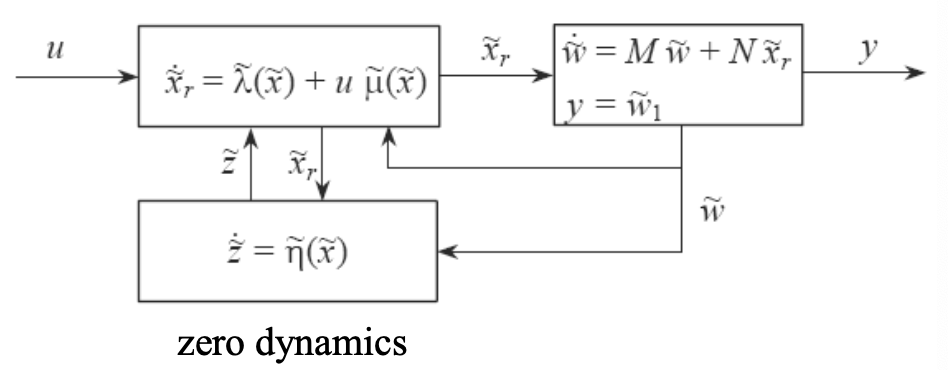
\includegraphics[scale=0.4]{immagini/zero_dyn}
	\caption{}
	\label{fig:zerodyn}
\end{figure}
\section{Normal canonical form for a linear system} \label{canonical}
We want to apply the method we have already studied to put a system in normal canonical form to a linear  system. The reason we do this is not for design feedback control  but to  understand how to check the fact that by applying feedback linearization you can actually stabilize your nonlinear system around an equilibrium.\\Let's start considering a linear dynamical system of order n, reachable and observable
\[S_L\colon \begin{cases}
	\dot{x}=Ax+Bu\\
	y=Cx
\end{cases}
\] and $G(s)=C(sI-A)^{-1}B$. Let $r<n$ be its relative degree. Then,\[
G(s)=\frac{\beta_rs^{n-r}+\beta_{r+1}s^{n-r-1}+\dots+\beta_{n-1}s+\beta_n}{s^n+\alpha_1s^{n-1}+\dots+\alpha_{n-1}s+\alpha_n}, \qquad \beta_r\neq0
\]

Without loss of generality we can suppose that the system is in controllable canonical form, that is
\begin{equation*}
A:=\begin{bmatrix}
	0 & 1 & 0 & \dots & 0 \\
	0 & 0 & 1 &  \dots & 0 \\
	0 & 0 & 0 & 0 & 0 \\
	\vdots& \vdots & \vdots & \vdots & \vdots \\
	0& 0 & 0 & 0 & 1 \\
	-\alpha_n &-\alpha_{n-1} & -\alpha_{n-2} & \dots & -\alpha_1 
\end{bmatrix}\quad 
B:=\begin{bmatrix}
0	\\
0	\\
0	\\
\vdots\\
	0\\
	1
\end{bmatrix}
\end{equation*}
\[C:=\begin{bmatrix}
	-\beta_n&-\beta_{n-1}  & \dots &-\beta_r  & 0 &0  & \dots & 0 
\end{bmatrix}
\]
What we will find out is that when you put a linear system in normal canonical form to apply the standard feedback linearizing control law, which make no sense since the system is already linear, you are going to isolate the part of the zero dynamic. The eigenvalues of this part are the zeros of G(s). So if the system is in non minimum phase, by putting the system in normal canonical form the zero dynamic will result unstable.
Let's perform a change of coordinate in an equivalent way as we did in Section \ref{changeofcoord}.
\[
\begin{cases}
	\dot{x}=Ax+Bu\\
	y=Cx
\end{cases} \xrightarrow{\tilde{x}=\varphi(x)}
\begin{cases}
	\dot{\tilde{x}}=\tilde{a}(\tilde{x})+\tilde{b}(\tilde{x})u\\
	y=\tilde{c}(\tilde{x})
\end{cases} 
\]
Given that the relative degree of $S_L$ is $r<n$, then, we can set $\varphi_k\colon=L_a^{k-1}c,\qquad k=1,2,\dots,r$. Since $a(x)=Ax,	\qquad b(x)=B,\qquad c(x)=Cx$:	\[
\varphi_1=L_a^0c=c \Rightarrow 	\varphi_1(x)=Cx=\beta_nx_1+\beta_{n-1}x_2+\dots+\beta_rx_{n-r+1}
\] In consequence:\[
L_a^1c=L_a\varphi_1 \Rightarrow \varphi_2(x)=CAx=\beta_nx_2+\beta_{n-1}x_3+\dots+\beta_rx_{n-r+2}
\]
\begin{equation*}
	Av:=\begin{bmatrix}
		0 & 1 & 0 & \dots & 0 \\
		0 & 0 & 1 &  \dots & 0 \\
		\vdots& \vdots & \vdots & \vdots & \vdots \\
		0& 0 & 0 & 0 & 1 \\
		-\alpha_n &-\alpha_{n-1} & -\alpha_{n-2} & \dots & -\alpha_1 
	\end{bmatrix} 
	\begin{bmatrix}
		v_1	\\
		v_2	\\
		\vdots	\\
		v_{n-1}\\
		v_n
	\end{bmatrix}=
	\begin{bmatrix}
	v_2	\\
	v_3	\\
	\vdots	\\
	v_{n}\\
	\star
\end{bmatrix}
\end{equation*}
\begin{equation*}
	A^{k-1}x=
	\begin{bmatrix}
		x_k	\\
		x_{k+1}	\\
		\vdots	\\
		x_n\\
		\star\\
		\star
	\end{bmatrix}\qquad
	C:=\begin{bmatrix}
		-\beta_n&-\beta_{n-1}  & \dots &-\beta_r  & 0 &0  & \dots & 0 
	\end{bmatrix}
\end{equation*} beacuse of the particular structure of the matrix A we can see a ''shift'' in the index of the products element in the result.
So, inn the end:\[
L_a^{r-1}c=L_a\varphi_{r-1} \Rightarrow \varphi_2(x)=CA^{r-1}x=\beta_nx_r+\beta_{n-1}x_{r+1}+\dots+\beta_rx_n
\] We need the lemma that guarantee the existence of further functions which make $\phi$ a diffeomorphism and have the property that the Lie derivetive respect vector field v is 0.
\begin{lemma}[complementary sub-transformation]
	If S has relative degree $r<n$ in x°, then , there exists n-r functions $\varphi_{r+k},\quad k=1,2,\dots,n-r$, regular in some neighborhood of x°. and such that \begin{itemize}
		\item[tiny] $\varphi_x$ is non singular in x°, where $\varphi=\begin{bmatrix} \varphi_1 & \varphi_2 & 	\dots & \varphi_n
		\end{bmatrix}'$;
		\item[tiny] $L_b\varphi_{r+k}=0$ in some neighborhood of x°, for any $k=1,2,\dots,n-r$
	\end{itemize} 
\end{lemma}
We need to look for $n-r$, $k=1,2,\dots,n-r$ such that \begin{itemize}
	\item $\varphi_x(x°)$ non singular
	\item $L_b\varphi_{r+k}=0$, in a neighborhood of x°, for any $k=1,2,\dots,n-r$
\end{itemize}
We shall next show that one such a choice is \[
\varphi_{r+k}(x)=x_k \qquad k=1,2,\dots, n-r
\]In conclusion the final change of coordinates to obtain the normal canonical form is \[\tilde{x}=\varphi(x)=\varphi_xx\] which satisfies the first request of \emph{non singularity}. We next show that $L_b\varphi_{r+k}=0,$ for any $k=1,2,\dots,n-r$.\[
L_b\varphi_{r+k}(x)=\begin{bmatrix}
	0&\dots&0&1&0&\dots&0&0&\dots&0
\end{bmatrix}B=0
\] since \begin{equation*}
B:=\begin{bmatrix}
	0	\\
	0	\\
	0	\\
	\vdots\\
	0\\
	1
\end{bmatrix}
\end{equation*}
Finally, what we build shows that there is a mapping appropriate to put the system in controllable canonical form.
\section{Zero dynamics of a linear system}
The linear case is a particular case of the nonlinear one. We have a linear part wich are the first r-1 components with corresponding matrices M and N is fed by the r-th components which have an affine structure on u with coefficients different from 0 in this setup for $\tilde{x}°$. And then the zero dynamics which is not affected by u.
\[
\left.
\begin{aligned}
	& \begin{bmatrix} \tilde{x}_1 & \tilde{x}_2 & \dots & \tilde{x}_{r-1}\end{bmatrix} := \tilde{w}\\
	&  \begin{bmatrix} \tilde{x}_{r+1} & \tilde{x}_{r+2} & \dots & \tilde{x}_n\end{bmatrix}:=\tilde{z}
\end{aligned}
\right\rbrace\qquad 	\tilde{x}=  \begin{bmatrix} \tilde{w}' & \tilde{x}_r & \dots & \tilde{z}\end{bmatrix}'
\] 
\begin{equation*}
	\left\{
	\begin{array}{ll}	
		\dot{\tilde{w}}=M\tilde{w}+N\tilde{x}_r & \in \Re^{r-1}\\
		\dot{\tilde{x}}_r=\tilde{\lambda}(\tilde{x})+u\tilde{\mu}(\tilde{x}) & \in \Re \qquad,\qquad \tilde{\mu}(\tilde{x}°)\neq 0\\
		\dot{\tilde{z}}=\tilde{\eta}(\tilde{x})\\
		y=\tilde{w}_1 &
	\end{array}
	\right.	 M:=\begin{bmatrix}
		0 & 1 & 0 & \dots & 0 \\
		0 & 0 & 1 & \dots & 0 \\
		0 & 0 & 0 & \dots & 0 \\
		\dots & \dots & \dots & \dots & \dots \\
		0 & 0 & 0 & \dots & 1 \\
		0 & 0 & 0 & \dots & 0
	\end{bmatrix}
N:=\begin{bmatrix}
0 \\
0 \\
0 \\
\vdots \\
0 \\
1
\end{bmatrix}
\end{equation*}
\begin{figure}[H]
	\centering
	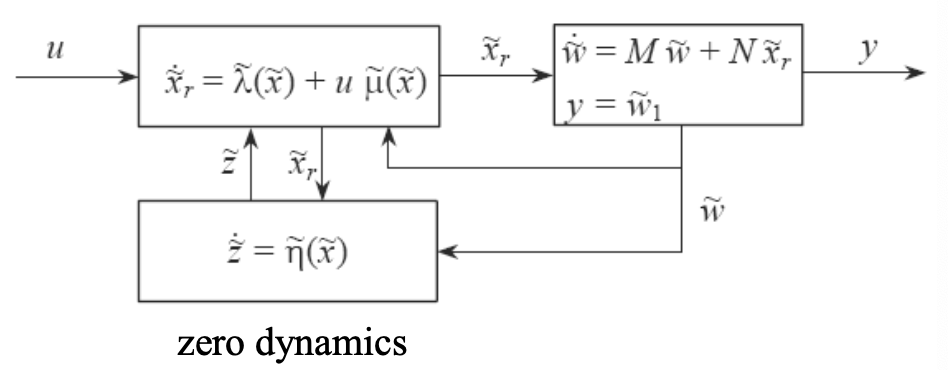
\includegraphics[scale=0.4]{immagini/zero_dyn}
\end{figure}
Since we are doing a linear transformation of a linear system the result is still linear:
\[
\dot{\tilde{x}}_r=L_a^rc+uL_bL_a^{r-1}c:=\lambda(x)+u\mu(x)=\tilde{\lambda}(\tilde{x})+u\tilde{\mu}(\tilde{x})
\]
\[
\dot{\tilde{x}}_r=CA^rx+CA^{r-1}Bu=CA^r\phi^{-1}_x
\tilde{x}+CA^{r-1}Bu\]We are missing the zero dynamics, the zero dynamics is $\tilde{z}_k=\phi_{r+k}(x)=x_k$ and since the system $S_L$ is in the controllable canonical form, then \[
\begin{aligned}
	& \dot{\tilde{z}}_1=\dot{x}_1=x_2=\tilde{z}_2\\
	&\dot{\tilde{z}}_2=\dot{x}_2=x_3=\tilde{z}_3\\
	\dots\\
	&\dot{\tilde{z}}_{n-r-1}=\dot{x}_{n-r-1}=x_{n-r}=\tilde{z}_{n-r}\\
	&\dot{\tilde}_{n-r}=\dot{x}_{n-r}=x_{n-r+1}
\end{aligned}
\]
By definition
\[
\phi_1(x)=Cx=\beta_nx_1+\beta_{n-1}x_2+\dots+\beta_rx_{n-r+1} \quad \text{and} \quad \phi_1(x)=\tilde{x}_1=\tilde{w}_1 
\]
Hence, $x_{n-r+1}=\frac{1}{\beta_r}(\tilde{w}_1-\beta_nx_1-\beta_{n-1}x_2-\dots-\beta_{r+1}x_{n-r})$ from which we get 
\[
x_{n-r+1}=\frac{1}{\beta_r}(\tilde{w}_1-\beta_n\tilde{z}_1-\beta_{n-1}\tilde{z}_2-\dots-\beta_{r+1}\tilde{z}_{n-r})
\]
\begin{equation*}
	\left\{
	\begin{array}{ll}	
		\dot{\tilde{w}}=M\tilde{w}+N\tilde{x}_r\\
		\dot{\tilde{x}}_r=\tilde{\lambda}(\tilde{x})+u\tilde{\mu}(\tilde{x}) & CA^{r-1}B \neq 0\\
		\dot{\tilde{z}}=F\tilde{z}+H\tilde{w}_1\\
		y=\tilde{w}_1
	\end{array}
	\right.
\end{equation*}
where
\begin{equation*}
	F:=\begin{bmatrix}
		0 & 1 & 0 & \dots & 0 \\
		0 & 0 & 1 & \dots & 0 \\
		0 & 0 & 0 & \dots & 0 \\
		\dots & \dots & \dots & \dots & \dots \\
		0 & 0 & 0 & \dots & 1 \\
		-\frac{\beta_n}{\beta_r} & -\frac{\beta_{n-1}}{\beta_r} & -\frac{\beta_{n-2}}{\beta_r} & \dots & -\frac{\beta_{r+1}}{\beta_r}
	\end{bmatrix}\quad
H:=\begin{bmatrix}
	0 \\
	0 \\
	0 \\
	\vdots \\
	0 \\
	\frac{1}{\beta_r}
\end{bmatrix}
\end{equation*}
\[
\beta_r \, det(sI-F)=\text{numerator of }G(s)=\frac{\beta_rs^{n-r}+\beta_{r+1}^{n-r-1}+\dots+\beta_{n-1}s+\beta_n}{s^n+\alpha_1s^{n-1}+\dots+\alpha_{n-1}s+\alpha_n}
\]
The eiqenvalues of F are the zeros of G(s) $\to$ non-minimum phase linear systems have unstable zero dynamics.
\section{Feedback linearization and pole assignement for the regulation at an equilibrium}Let's go back in our case of interest
\[S_L\colon \begin{cases}
	\dot{x}=a(x)+b(x)u\\
	y=c(x)
\end{cases}
\] 
I/O feedback linearization can be performed in an arbitrary state x° for regularize the sytem, where the relative degree of system S is well-defined.
Our case of interest:\\
x° is an equilibrium associated with a constant input u of S. We aim at regulating S at such an equilibrium.\\
Assumption: the relative degree of S at x° is r\\
Without loss of generality, we assume that: $a(0) = 0, c(0) = 0$
which means that x° = 0 is an equilibrium obtained for u=0, and that the output at the equilibrium is zero.\\
Let us consider the change of coordinates $\tilde{x}:=L^{k-1}_ac,\quad k=1,2,\dots,r$ satisfy $\phi_k(0):=[L^{k-1}_ac]_0=0,\quad k=1,2,\dots,n-r$ so that the equilibrium x°=0 in the new coordinate is still zero:\[\tilde{x}°=\phi(x°)=\phi(0)=0\]
To sum up the new feedback linearizing control law is \[
u=\frac{1}{\tilde{\mu}(\tilde{x})}[v-\tilde{\lambda}(\tilde{x})]:=\tilde{\beta}(\tilde(x))[v-\tilde{\alpha}(\tilde{x})]
\]\begin{figure}[H]
	\centering
	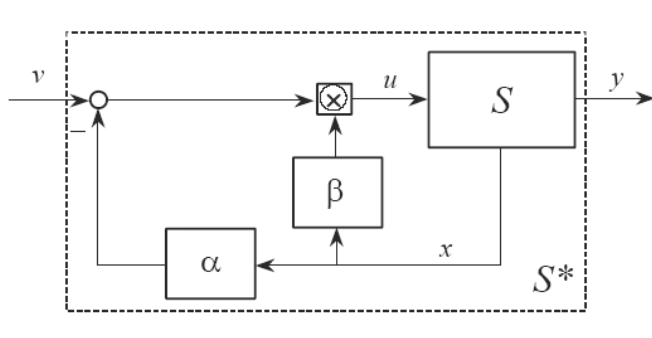
\includegraphics[scale=0.4]{immagini/finalu}
	\caption{}
	\label{fig:finalu}
\end{figure}
So the closed-loop system in the new coordinate results:
\begin{equation*}
	\left\{
	\begin{array}{ll}	
		\dot{\tilde{w}}=M\tilde{w}+N\tilde{x}_r & \in\Re^{r-1}\\
		\dot{\tilde{x}}_r=v & \in \Re\\
		\dot{\tilde{z}}=\tilde{\eta}(\tilde{x}) & \in \Re{n-r}\\
		y=P\tilde{w} & \in \Re
	\end{array}
	\right.
\end{equation*} where $P':=\begin{bmatrix}
1 & 0 & 0 & \dots & 0
\end{bmatrix}'\,\in\Re^{r-1}$.\\
So for what concern the linear part it's isolated here by uncluding in q also the $\tilde{x}_r$ varibale added to the w. This not yet asymptotically stable because it's an integrator of order r. Reasoning on the subsystem representing the linear part is however reachable and observable because if we determine the transfer funcitons $G(s)=\frac{1}{s^r}$, it has exactly r poles, with r that is  te number of $\tilde{w}$ variable.
\[
\tilde{q}:=\begin{bmatrix}
	\tilde{w}\\
	\tilde{x}_r
\end{bmatrix}, \quad A:= \begin{bmatrix}
M & N \\
0 & 0
\end{bmatrix}, \quad B:=\begin{bmatrix}
0 \\
1
\end{bmatrix}, C:=\begin{bmatrix}
P' & 0
\end{bmatrix}
\]The system splitted between linear part and zero dynamic is as follows
\begin{equation*}
	\left\{
	\begin{array}{ll}	
		\dot{\tilde{q}}=A\tilde{q}+Bv\\
		y=C\tilde{q}\\
		\boxed{\dot{\tilde{z}}=\tilde{\eta}(\tilde{x})}\\
	\end{array}
	\right.
\end{equation*} Where $\dot{\tilde{z}}$ is the hidden dynamics generated by the state feedback linearizing control law.\\Now we have to problems: first one is that we have to stabilize the linear part, and then make some consideration on what kind of properties we can guarantee and how we can analyze the contribution of the hidden dynamic. It's not contributing to the output but it is contribuiting to the stability properties.
\begin{figure}[H]
	\centering
	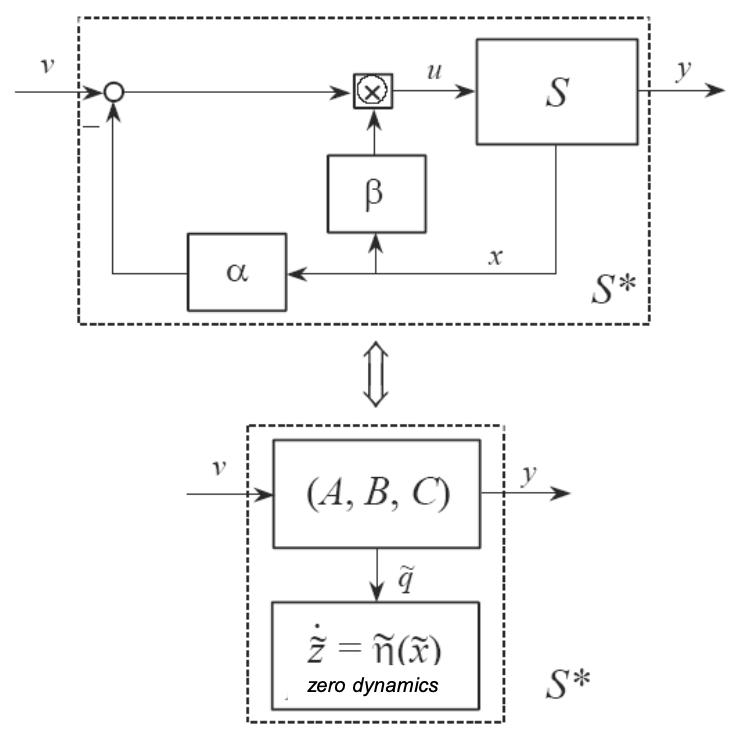
\includegraphics[scale=0.4]{immagini/big_scheme}
	\caption{}
	\label{fig:bigscheme}
\end{figure}
Our final objective is to regularize the system around ur new equilibrium $\tilde{x}°$ which is the equilibrium x°=0 associated with u=0. We can notice that the zero equilibrium in the original coordinates associated wiht input u=0 is actually mapping
in a zero equilibrium for the new input v=0. So $\tilde{x}°$ is an equilibrium of the feedback linearized system associated with input $v \equiv 0$. So what we have to do now is to make that equilibirum asymptotically stable. Forgetting about the hidden part this will be very easy beacuse it is a linear system which is controllable, so we can apply the standard linear static state feedback in $\tilde{q}$. Setting $v=-K\tilde{q}+v$ with $\begin{pmatrix}
	k_r & k_{r-1} & \dots & k_1
\end{pmatrix}$ where $\tilde{q}$ are the first components of $\tilde{x}(t)=\phi(x(t))$ we then get: 
\begin{equation*}
	\left\{
	\begin{array}{ll}	
		\dot{\tilde{q}}=(A-BK)\tilde{q}+Bv\\
		y=C\tilde{q}\\
		\dot{\tilde{z}}=\tilde{\eta}(\tilde{x})\\
	\end{array}
	\right.
\end{equation*}\[
\begin{bmatrix}
	0 & 1 & 0 & \dots & 0 \\
	0 & 0 & 1 & \dots & 0 \\
	\dots & \dots & \dots & \dots & \dots \\
	0 & 0 & 0 & \dots & 1 \\
	-k_r & -k_{r-1} & -k_{r-2} & \dots & -k_1
\end{bmatrix} 
\] The linear part (A-BK,B,C) is in the controllable form, reachable and observable, with a transfer function with no zeros and poles given by the roots of the characteristc polynomial of matrix A-BK: \[
\chi(s)=s^r+k_1s^{r-1} + k_2s^{r-2}+\dots+k_r
\] we can chose the coefficient to put the polese wherever we want.
\subsection{Feedback linearization with pole assignment}
So at the very end our u variable is:\[
	u=\tilde{\beta}(\tilde{x})[v-\tilde{\alpha}(\tilde{x})]=\tilde{\beta}(\tilde{x})[v-\tilde{\gamma}\tilde{x}-\tilde{\alpha}(\tilde{x})]=\beta(x)[v-\tilde{\gamma}\phi(x)-\alpha(x)]
\] obtained sobstituiting in place of v, the part that stabilize the linear subpart of the system in the normal form which is $v=-K\tilde{q}+v \quad \tilde{\gamma}:=[K \, 0]$. We use $\tilde{\gamma}$ because we need to extend K with the 0.
\begin{figure}[H]
	\centering
	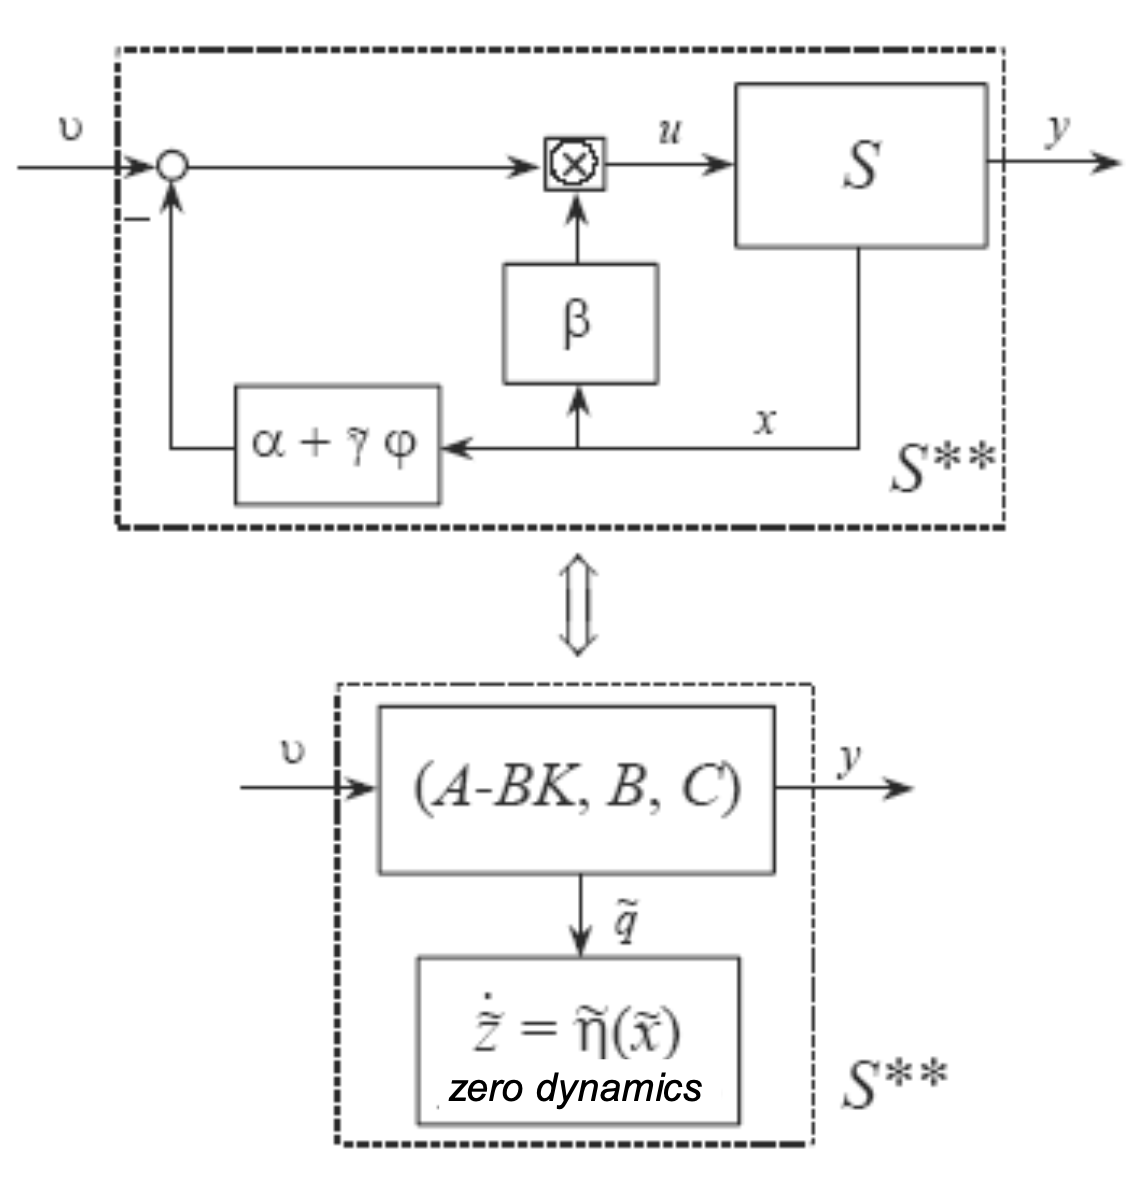
\includegraphics[scale=0.4]{immagini/f_lin_with_pass}
	\caption{}
	\label{fig:flinwithpass}
\end{figure}
Now we can have to cases: if \textcolor{red}{r=n} in the normal canonical form description in the $\tilde{x}$	variable we will have a asymptotically stable linear system	while if \textcolor{red}{r$<$n} we have a zero dynamics that we have to account for in order to asses if $\tilde{x}°=0$ is indeed asymptotically stable.
The zero dynamic is fed only by a subpart of the states and does not depend on the input but only from the state $\tilde{q}$. The input of zero dyanamic $\tilde{q}$ is going to zero equilibrium ($\tilde{q}\to0$) because we impose asymptotic stability, as the associated zero imput equilibrium. We need to know now what happens when the zero dynamics is fed by an input that goes asymptotically to zero.\\
If we know the expression of the zero dynamics, and if it is linear we can just analyze the eigenvalues and check if the dyanamic matrix of the system is Hurwitz. But if this is not the case and the full linearization is not possible, then
the I/O linearization $S^*$ of systems $S$ around the origin with pole assignment is not meaningful if $\tilde{z}=0$ is not an asymptotically stable equilibrium of the zero dynamics associated with $\tilde{q}=0$  , with a suitable domain of attraction. The results goes as follows:
\begin{equation*}
	\left\{
	\begin{array}{ll}	
		\dot{x}=a(x)+b(x)u\\
		y=c(x)\\
	\end{array}
	\right. \qquad a(0)=0;\, c(0)=0
\end{equation*}
The goal is to regularize around the zero equilibrium associated with the zero input, in order to see if feedback linearization can work effectivley we first check if the relative degree is well defined (r=n). But if r<n how do we now if the whole process makes sense and the zero dyanic is asymptotically stable? We build the linear tangent model to S in x°=0:
$\delta S:$\begin{equation*}
	\left\{
	\begin{array}{ll}	
		\delta \dot{x}=a_x(0)\delta x+b(0)\delta u
		\delta y=c_x(0)\delta x\\
	\end{array}
	\right. \qquad G_0(s):=c_x(0)[sI-a_x(0)]^{-1}b(0)
\end{equation*}
\begin{prop}
 Let $r$ be the relative degree of S in x°. Then,
 \begin{itemize}
 	\item the relative degree of $G_0(s)$ is equal to r;
 \end{itemize}
If we denote with $F:=\tilde{\eta}_{\tilde{z}}(0)$ the Jacobian in the orign of the zero dynamics of S, then, 
\begin{itemize}
	\item the eigenvalues of F are the zeros of $G_0(s)$
\end{itemize}
\end{prop}
 This proposition is particularly useful becasue if we build a tangent model, compute the transfer function, and if the transfer function is minimum phase then we are sure that the zero dynamic is locally asympototically stable at the equilibrium. 
 We can then a-priori verify if the I/O feedback linearization is sound, at least locally, by assessing the stabilizability of $\delta S$ and that the zeros of $G_0(s)$ have negative real part.
 \subsection{State feedback full linearizability problem}
 How can we choose the output c(x) to get relative degree r equal to the order of the system?\\
 The problem now is a bit different because we start from a system where the outmap is not defined because i'm looking for if exists one that guarantees r=n.
 \[S_0:\quad \dot{x}=a(x)+b(x)u\] with $a(0)=0, \, b(0)\ne0$ and fully measurable state, determine if (and how) one cas design, locally to x°=0, a diffeomorphism $\phi$ with $\phi(0)=0$, and a state feedback law \[u=\beta(x)v+\sigma(x)\] such that in the new coordinates $\tilde{x}=\phi(x)$ the closed-loop system takes the linear form \[S^*_0: \quad \dot{\tilde{x}}=A\tilde{x}+Bv\] with (A,B) reachable.\\
 \underline{Known fact}: There exists a solution to the state feedback full linearizability problem in x°=0 if one can find a regular function $c(\cdot)$ with c(0)=0 such that
 \begin{equation*}
 	\left\{
 	\begin{array}{ll}	
 		\dot{x}=a(x)+b(x)u\\
 		y=c(x)
 	\end{array}
 	\right. \qquad a(0)=0;\, c(0)=0
 \end{equation*}
 has relative degree r equal to the order n of the system in x°=0.\\
 Then, the state feedback control law which is fully linearizing the system exists. So it is a sufficient condition. But in fact can be proven that is also a necessary condition!
 \begin{thm}
 	There exists a solution to the state feedback full linearizability problem in x°=0 \underline{if and only if} one can find a regular function $c(\cdot)$ with c(0)=0 such that system
 	 \begin{equation*}
 		\left\{
 		\begin{array}{ll}	
 			\dot{x}=a(x)+b(x)u\\
 			y=c(x)
 		\end{array}
 		\right. \qquad a(0)=0;\, c(0)=0
 	\end{equation*} has relative degree r equal to the order n of the system in x°=0.
 \end{thm}
What is the practical impact of this theorem? What we could do is looking, searching, trying to compute a c(x) output map. We have to compute a feasibility analysis reguarding the existance of a regular function $c(\cdot)$ that satisfies the following relations:
 	 \begin{equation*}
	\left\{
	\begin{array}{ll}	
		L_Bc=0\\
		L_bL_ac=0\\
		\vdots\\
		L_bL_a^{n-2}c=0
	\end{array}
	\right.
\end{equation*} in a neighborhood of x°, and $[L_bL_a^{n-1}c]_{x°}\neq0]$. Once the existance of the solution is stated we can find a solution to n - 1 nonlinear partial differential equations. But now we want to make some conditions in order to proove the existance of a solution without too much effort.\\
The existence of \textcolor{red}{$c(x)$ can be characterized by necessary and sufficient conditions} on the vector fields $a(x)$ and $b(x)$.
We need first to introduce some terminology.\\
\begin{defn}[Lie Bracket]
	given two vector fields $a,b:D\to\Re^n$ with $D\subseteq\Re^n$, the Lie Bracket of a and b is the vector field $[a,b]:D\to\Re^n$ given by \[
	[a,b]=\frac{\partial b}{\partial x}a-\frac{\partial a }{\partial x}b=L_ab-L_ba
	\]Note that $a\equiv b\equiv\text{constant}\Rightarrow[a,b]=0$.\\The Lie Bracket [a,b] is commonly written as $ad_ab$ where ad stands for 'adjoint'. Repeated Lie Brackets can be defined recursivly by
	\[
	\begin{aligned}
		&ad_a^0b=b\\
		&ad_a^1b=[a,ad_a^0b]=[a,b]\\
		&ad_a^ib=[a,ad_a^{i-1}b],\, i=\,2,\dots
	\end{aligned}
	\]
\end{defn}
\begin{thm}
	The state feedback full linearizability problem has a solution if and only if there exists an open set $D, \, x°\in D$, such that the following conditions hold:
	\begin{enumerate}
		\item Vectors ${b(x),ad_a^1b(x),\dots,ad_a^{n-1}b(x)}$ are linearly independent for all $x\in D$
		\item The set of vector fields ${b,ad_a^1b,\dots,ad_a^{n-2}b}$ is involutive in D
	\end{enumerate}
\end{thm}
\begin{defn}
	Let $f:D\to\Re^n$ with $D\subseteq\Re^n$ be a regular vector field, $i=1,\dots,m$. The set ${f_1,f_2,\dots,f_m}$ is involutive if \[
	rank\begin{bmatrix}
		f_1(x) & f_2(x) & \dots & f_m(x)
	\end{bmatrix}=rank\begin{bmatrix}
	f_1(x) & f_2(x) & \dots & f_m(x) & [f_i(x),\, f_j(x)]
\end{bmatrix}
	\]
	for all $x\in D$ and $i,j \in {1,2,\dots,m}$.
\end{defn}
\begin{remark}
	\begin{itemize}
		\item The first condition can be interpreted as controllability condition for the nonlinear system;
		\item The involutivity condition is less intuitive. It is trivially satisfied for linear systems, but not generally satisfied in the nonlinear case.
	\end{itemize}
\end{remark}
In the end, the input-state linearization problem in $x°$ can be addressed as follows:
\begin{enumerate}
	\item  Construct the vector fields ${b,ad_a^1b,\dots,ad_a^{n-1}b}$ for the given regular
	system
	\item Check whether the controllability and involutivity conditions are
	satisfied in $D$ containing $x°$
	\item If both conditions are satisfied, find the output function $c(x)$ which
	will lead to the input-output linearization solving
	 \begin{equation*}
		\left\{
		\begin{array}{ll}	
			L_Bc=0\\
			L_bL_ac=0\\
			\vdots\\
			L_bL_a^{n-2}c=0
		\end{array}
		\right.
	\end{equation*} in a neighborhood of x°, and $[L_bL_a^{n-1}c]_{x°}\neq0]$.
\end{enumerate}
